\section{Amplitude Formalism}

Now we embark on the topic of amplitudes. We wish to describe the dynamics of our reaction in a way that allows us to extract quantum numbers like spin from our data. There are several difficulties in doing so: First, we are trying to determine the properties of many particles at once, and we know that many resonances in this channel overlap in mass space. This precludes the use of a simple Breit-Wigner description of most of these resonances, as overlapping Breit-Wigners do not preserve unitarity. Second, the GlueX experiment uses a linearly polarized photon beam, so it behooves us to use a formalism which can include this polarization. Finally, there are many resonances in this channel, and while we have the largest photoproduction dataset to date, we are still relatively data limited, which further complicates any dynamical description. The majority of this section is a summary of the formalisms described in~\cite{Chung1971} and~\cite{Richman1984}.

\subsection{Single-Particle Helicity States}

We begin by defining a set of observables which are independent of frames and rotations on those frames. This is known as the helicity formalism, where helicity resembles the spin projection along the axis of a particle's motion. First, we define a rotation $R(\alpha, \omega, \gamma)$ as a matrix whose action on a vector is a rotation about the Euler angles $\alpha$, $\omega$, and $\gamma$. For each rotation, we can define a unitary operator $U[R]$ which has the group property $U[R_2 R_1] = U[R_2] U[R_1]$ as it is an operator on the group $SO(3)$. Being an operator on $SO(3)$, we can also write it as

\begin{equation}
  U[R(\alpha,\omega,\gamma)] = e^{-\imath \alpha J_z} e^{-\imath \omega J_y} e^{-\imath \gamma J_z}.
  \label{eq:rotation-rep}
\end{equation}

We can then describe the matrix elements of this operator in the angular momentum eigenbasis $\ket{jm}$ (representing a spin-$j$ particle where $m$ is the projection of spin onto the $\hat{z}$-axis) with the Wigner D-matrix:

\begin{gather}
  U[R(\alpha, \omega, \gamma)] \equiv \sum_{m'} \ket{jm} D_{m'm}^j(R(\alpha, \omega, \gamma)), \\
  \text{where} \notag\\
  D_{m'm}^j(\alpha, \omega, \gamma) \equiv e^{-\imath m' \alpha} d_{m'm}^j e^{-\imath m\gamma} \\
  \text{and} \notag\\
  d_{m'm}^j(\omega) = \mel{jm'}{e^{-\imath\omega J_y}}{jm}.
  \label{eq:wigner-d-definition}
\end{gather}

We can further extend this eigenbasis to include linear momentum by introducing Lorentz boosts $L(\vec{\beta})$. We denote the operation of a boost along the $\hat{z}$-axis with velocity $\beta$ as $L_z(\beta)$. A boost in any direction described by polar angles $(\theta, \varphi)$ can be achieved by rotating the $\hat{z}$-axis to align with the direction vector, boosting in the new $\hat{z}$-direction, and rotating back:

\begin{equation}
  L(\vec{\beta}) = R(\varphi, \theta, 0) L_z(\beta) R^{-1}(\varphi,\theta,0)
\end{equation}

Together, the space of rotations and boosts defines the Lorentz group, where each arbitrary Lorentz transformation $\Lambda$ has a unitary operator $U[\Lambda]$ with the group property $U[\Lambda_2 \Lambda_1] = U[\Lambda_2]U[\Lambda_1]$, so in terms of operators, we can also write

\begin{equation}
  U[L(\vec{p})] = U[R(\varphi, \theta, 0)]U[L_z(p)]U^{-1}[R(\varphi,\theta,0)].
\end{equation}

Finally, this allows us to define the ``canonical'' basis for a single particle as
\begin{equation}
  U[L(\vec{p})]\ket{jm} \equiv \ket{\vec{p},jm}.
  \label{eq:canonical-single-particle}
\end{equation}

Unfortunately, the quantum number $m$ is only valid in the rest frame of the state because the $\hat{z}$-axis of the rest frame is not equivalent to the $\hat{z}$-axis in any arbitrarily Lorentz-transformed frame. Therefore, we will define helicity $\lambda$ as the projection of spin along the direction of motion and introduce new helicity states,

\begin{equation}
  \ket{\vec{p},j\lambda} = U[L(\vec{p})]U[R(\varphi,\theta,0)]\ket{j\lambda} = U[R(\varphi,\theta,0)]U[L_z(p)]\ket{j\lambda}.
  \label{eq:helicity-single-particle}
\end{equation}

In this definition, we have two ways of obtaining the helicity frame: We can either rotate the state first such that the quantization axis is aligned with $\vec{p}$ and then boost in the $\hat{p}$-direction or we can first boost in the $\hat{z}$-direction and then rotate. In either equivalent case, $\lambda$ is invariant under rotations as well as boosts parallel to $\vec{p}$. Finally, we can define these helicity states over a basis of canonical states:

\begin{equation}
  \ket{\vec{p},j\lambda} = \sum_m D_{m\lambda}^j(R(\varphi, \theta, 0)) \ket{\vec{p}, jm}.
  \label{eq:canonical-to-helicity}
\end{equation}

The single-particle states are normalized such that

\begin{gather}
  \bra{\vec{p}',j'\lambda'}\ket{\vec{p},j\lambda} = \tilde{\delta}(\vec{p}' - \vec{p})\delta_{j'j}\delta_{\lambda'\lambda} \\
  \text{with } \tilde{\delta}(\vec{p}' - \vec{p}) = (2\pi)^3(2E)\delta^{(3)}(\vec{p}'-\vec{p}), \notag
  \label{eq:helicity-normalization}
\end{gather}
since the Lorentz-invariant phase space element is given by $\tilde{\dd{p}} = \frac{\dd[3]{\vec{p}}}{(2\pi)^3(2E)}$. This gives the following representation of the identity:

\begin{equation}
  \sum_{j\lambda}\int \ket{\vec{p},j\lambda}\tilde{\dd{p}}\bra{\vec{p},j\lambda} = I
\end{equation}

\subsection{Two-Particle Helicity States}

Of course, we would like to extend these states to be able to talk about interactions and decays. For notation, I will use $\Omega$ to represent the polar angles $\theta$ and $\varphi$ and $\varnothing$ to describe the specific value of $0$ for both of these angles. Similarly, $R_\Omega$ and $R_\varnothing$ will represent the corresponding rotation operators (the second being a null rotation the direction of the $\hat{z}$-axis). $R$ without subscript or angles will represent an arbitrary rotation whose angles are not important for the derivation.

Next, we can define a joint state of two particles with masses $w_1$ and $w_2$ (to avoid confusion with angular moments) and spins $s_1$ and $s_2$. In the center-of-momentum (COM) frame, these particles are back-to-back, and we can define the momentum of particle 1 as $\vec{p}$ with direction $\Omega$ and particle 2 as $-\vec{p}$. Then the joint canonical state, up to a normalization constant $\mathcal{N}$, is given by

\begin{equation}
  \ket{\Omega,s_1m_1s_2m_2} = \mathcal{N} U[L(\vec{p})]\ket{s_1m_1} U[L(-\vec{p})]\ket{s_2m_2}.
  \label{eq:two-particle-canonical}
\end{equation}

Such a state can also be described with a total spin $s$ and spin projection $m_s$:

\begin{equation}
  \ket{\Omega, sm_s} = \sum_{m_1m_2} \left(s_1m_1s_2m_2\mid sm_s\right)\ket{\Omega,s_1m_1s_2m_2}.
\end{equation}

Here, $\left(s_1m_1s_2m_2\mid sm_s\right)$ is the Clebsch-Gordan coefficient describing the angular momentum coupling. Next, we can add additional angular momentum apart from the spin. For a system with angular momentum $\ell$ with moment $m$, we use the fact that $\bra{\Omega}\ket{\ell m} = Y_{\ell}^m(\Omega)$ (spherical harmonics) to define

\begin{equation}
  \ket{\ell m s m_s} = \int \dd{\Omega} Y_{\ell}^m(\Omega) \ket{\Omega; s m_s}.
  \label{eq:two-particle-canonical-angular-momentum}
\end{equation}

Next, the spin $s$ and angular momentum $\ell$ can be coupled into the total angular momentum $J$ with moment $M$:

\begin{equation}
  \ket{J M \ell m s m_s} = \sum_{m\,m_s} \left(\ell m s m_s \mid JM\right)\ket{\ell m s m_s}.
  \label{eq:two-particle-canonical-total-angular-momentum}
\end{equation}

This coupled state is still in the canonical formalism, and we would like to use the helicity basis. Using \Cref{eq:helicity-single-particle},

\begin{equation}
  \ket{\Omega,s_1\lambda_1 s_2\lambda_2} = \mathcal{N} U[R_\Omega] \underbrace{\left(U[L_z(p)]\ket{s_1\lambda_1} U[L_{-z}(p)]\ket{s_2,-\lambda_2}\right)}_{\ket{\varnothing, s_1\lambda_1 s_2\lambda_2}}.
  \label{eq:two-particle-helicity}
\end{equation}

To obtain states with a total angular momentum, we can integrate over the space of all rotations, weighted by Wigner D-matrices:

\begin{equation}
  \ket{JM s_1\lambda_1 s_2\lambda_2} = \frac{N_J}{2\pi} \int \dd{R} D_{M\mu}^{J*}(R) U[R]\ket{\varnothing, s_1\lambda_1 s_2\lambda_2}
\end{equation}

This is, of course, incomplete, as we have not defined the normalization factor $N_J$ or the coupling $\mu$ which relates helicities to total angular momentum. To do both, let us specify the rotation $R$ as follows:

\begin{align}
  \ket{JM s_1\lambda_1 s_2\lambda_2} &= \frac{N_J}{2\pi}\int \dd{R} D_{M\mu}^{J*}(R) U[R(\varphi, \theta, \gamma)]\ket{\varnothing, s_1\lambda_1 s_2\lambda_2} \notag \\
                                     &= \frac{N_J}{2\pi}\int \dd{R} D_{M\mu}^{J*}(R) U[R(\varphi, \theta, 0)]U[R(0, 0, \gamma)]\ket{\varnothing, s_1\lambda_1 s_2\lambda_2} \notag \\
                                     &= \frac{N_J}{2\pi}\int \dd{R} D_{M\mu}^{J*}(R) e^{-\imath (\lambda_1 - \lambda_2)\gamma}U[R(\varphi, \theta, 0)]\ket{\varnothing, s_1\lambda_1 s_2\lambda_2} \notag \\
                                     &= \frac{N_J}{2\pi}\int \dd{\Omega}\dd{\gamma} e^{\imath M \varphi} d^{J*}_{M\mu} e^{\imath \mu \gamma} e^{-\imath (\lambda_1 - \lambda_2)\gamma}U[R(\varphi, \theta, 0)]\ket{\varnothing, s_1\lambda_1 s_2\lambda_2} \notag \\
                                     &= \frac{N_J}{2\pi}\int \dd{\Omega}\dd{\gamma} e^{\imath M \varphi} d^{J*}_{M\mu} e^{\imath (\mu - (\lambda_1 - \lambda_2)) \gamma} \ket{\Omega, s_1\lambda_1 s_2\lambda_2} \notag \\
                                     &= N_J\int \dd{\Omega} D_{M\lambda}^{J*}(R_{\Omega}) \ket{\Omega, s_1\lambda_1 s_2\lambda_2} \\
                                     &\text{with } \lambda = \lambda_1 - \lambda_2 \notag
\end{align}

It can be shown that the normalization is $\mathcal{N} = \frac{1}{4\pi} \sqrt{\frac{p}{\sqrt{s}}}$ where $p$ is the relative momentum and $\sqrt{s}$ the center-of-momentum energy the two-particle system ($s$ is the Mandelstam variable). The normalization of the standard two-particle states is given by

\begin{equation}
  \bra{\Omega', s'_1\lambda'_1 s'_2\lambda'_2}\ket{\Omega, s_1\lambda_1 s_2\lambda_2} = \delta^{(2)}(\Omega' - \Omega) \delta_{s'_1 s_1} \delta_{\lambda'_1\lambda_1} \delta_{s'_2 s_2} \delta_{\lambda'_2\lambda_2}.
\end{equation}

This follows immediately from \Cref{eq:helicity-normalization}. Next, to ensure that

\begin{equation}
  \bra{J'M' s'_1\lambda'_1 s'_2\lambda'_2}\ket{JM s_1\lambda_1 s_2\lambda_2} = \delta_{J'J} \delta_{M'M} \delta_{s'_1 s_1} \delta_{\lambda'_1\lambda_1} \delta_{s'_2 s_2} \delta_{\lambda'_2\lambda_2},
\end{equation}
we must have $N_J = \sqrt{\frac{2J+1}{4\pi}}$. Finally,

\begin{equation}
  \bra{\Omega, s'_1\lambda'_1 s'_2\lambda'_2}\ket{JM s_1\lambda_1 s_2\lambda_2} = N_J D_{M\lambda}^{J*}(R_\Omega) \delta_{s'_1 s_1} \delta_{\lambda'_1\lambda_1} \delta_{s'_2 s_2} \delta_{\lambda'_2\lambda_2}.
  \label{eq:angular-momentum-angle-coupling}
\end{equation}

\subsection{Production Amplitudes}\label{sub:production-amplitudes}

Given the two-particle helicity states, we can now construct production amplitudes which will model what we measure in the experiment.

We approach this with the $S$-matrix formalism. We assert that all of the dynamics of any reaction $i \to f$ are elements of an invariant scattering matrix $S$ written $\mel{f}{S}{i}$. We then define the matrix $T$ such that $S = 1 + 2 \imath T$, called the transition matrix\footnote{The factor of $2\imath$ here is purely convention and makes some derivations more compact.}.

Let us examine the reaction $a + b \to c + d$. We can write the invariant $S$-matrix element as

\begin{equation}
  \mel{\vec{p}_c\lambda_c;\vec{p}_d\lambda_d}{S}{\vec{p}_a\lambda_a;\vec{p}_b\lambda_b} = (4\pi)^2 \sqrt{\frac{s}{p_fp_i}}\mel{\Omega\lambda_c\lambda_d}{S(\sqrt{s})}{\varnothing\lambda_a\lambda_b},
  \label{eq:s-matrix-abcd}
\end{equation}
where we have used \Cref{eq:two-particle-helicity} to write the states with an initial momentum $(-)\vec{p}_i$ for particle ($b$)$a$ pointing along the direction $(\theta,\varphi) = (0,0) \equiv \varnothing$ and a final momentum $(-)\vec{p}_f$ for particle ($d$)$c$ pointing in the direction $\Omega$ with respect to $\vec{p}_i$. We can replace $S$ with the definition of $T$ to arrive at a similar formula for the invariant transition amplitude $\mathcal{M}_{fi}$:

\begin{equation}
  \mathcal{M}_{fi} = (4\pi)^2 \sqrt{\frac{s}{p_fp_i}}\mel{\Omega\lambda_c\lambda_d}{T(\sqrt{s})}{\varnothing\lambda_a\lambda_b}
  \label{eq:transition-amplitude}
\end{equation}

While we will not measure a cross-section in this experiment, we will roughly measure the number of events as a function of mass and helicity angles, which is proportional to the cross section. We refer to this as the ``intensity'' function (see Appendix B of~\cite{Chung1971}),

\begin{equation}
  I(m, \Omega) \propto \pdv{\sigma}{m}{\Omega} \equiv \frac{p_f}{p_i}\abs{\frac{\mathcal{M}_{fi}}{8\pi\sqrt{s}}}^2.
  \label{eq:intensity-definition}
\end{equation}

We can also use this formalism to model two-body decays of the form $X \to 1 + 2$, where $X$ has total angular momentum $J$. Starting in the rest frame of particle $c$, we say that particle ($2$)$1$ has momentum $(-)\vec{p}$, so the amplitude for a particular angular moment $M$ can be written as

\begin{align}
  \mel{\vec{p}\lambda_1;-\vec{p}\lambda_2}{\mathcal{M}}{JM} &= \bra{\vec{p}\lambda_1;-\vec{p}\lambda_2}\ket{JM\lambda_1\lambda_2}\bra{JM\lambda_1\lambda_2}\mathcal{M}\ket{JM} \\
                                                            &= 4\pi\sqrt{\frac{w}{p}}\underbrace{\bra{\Omega\lambda_1;-\vec{p}\lambda_2}\ket{JM\lambda_1\lambda_2}}_{N_J D_{M\lambda}^{J*}(\Omega)}\bra{JM\lambda_1\lambda_2}\mathcal{M}\ket{JM} \\
                                                            &\equiv N_J D_{M\lambda}^{J*}(\Omega) F^J_{\lambda_1\lambda_2},
  \label{eq:decay-amplitude}
\end{align}
where $w$ is the effective mass of the decaying particle, $\lambda = \lambda_1 - \lambda_2$, and we use the completeness relation,

\begin{equation}
\sum_{JM\lambda_1\lambda_2}\ket{JM\lambda_1\lambda_2}\bra{JM\lambda_1\lambda_2} = 1,
\end{equation}
along with \Cref{eq:angular-momentum-angle-coupling}. We call $F^J_{\lambda_1\lambda_2}$ the helicity decay amplitude.

If we wish to model $X \to K_S^0 K_S^0$, we first recognize that the kaon is a spin-$0$ particle, so the difference in helicity is $\lambda = 0$. Therefore,

\begin{equation}
  I(m,\Omega) \propto \abs{\mathcal{M}_{fi}}^2 \sim \abs{N_J D^{J*}_{M0}(\Omega) F^J(m)}^1 = \abs{Y_J^M(\Omega) F^J(m)}^2.
  \label{eq:decay-amplitude-intensity}
\end{equation}

Since we cannot know the spin projection of a particle \textit{a priori}, we will typically obtain it from fitting the intensity to a sum over these spherical harmonics, assigning an coefficient $a^J_M$ to each and determining the spin from the best-fitting harmonic,

\begin{equation}
  I(m,\Omega)\propto \abs{\sum_{JM}a^J_M F^J(m) Y_J^M(\Omega)}^2.
  \label{eq:partial-wave-expansion}
\end{equation}

It is important to remember here that $\Omega$ has always been defined in terms of the helicity angles of the decay, i.e. the spherical angles with respect to the direction of particle $X$'s motion found after boosting to the helicity frame. This frame is defined as the rest-frame of $X$ (found by boosting first from the lab frame to the center-of-momentum) with $\hat{z}$ defined as the boost direction from the center-of-momentum frame, $\hat{y}$ as normal to the production plane (the plane in which the beam and recoil proton move), and $\hat{x} = \hat{y}\cross\hat{z}$.

\subsection{Including Linear Photon Polarization}

Since the GlueX beam has a known polarization, we can take advantage of this extra information to explore the parity exchanged in our reaction. Mathieu et al.~\cite{Mathieu2019} provide a derivation which begins with a slightly different representation of the scattering matrix, written in terms of spin-density matrix elements $\rho^\gamma_{\lambda\lambda'}$ describing the coupling of a polarized photon to the helicity of the proton target (and that of the recoiling proton product):

\begin{equation}
  I(m,\Omega) \propto \frac{p_f}{p_i}\abs{\frac{\mathcal{M}_{fi}}{8\pi\sqrt{s}}}^2 = \kappa \sum_{\lambda\lambda'\lambda_p\lambda_{p'}} A_{\lambda;\lambda_p\lambda_{p'}}(m,\Omega)\rho^{\gamma}_{\lambda\lambda'}A^*_{\lambda';\lambda_1\lambda_2}(m,\Omega),
  \label{eq:intensity-sdme}
\end{equation}
where

\begin{equation}
  \kappa(m, s) = \frac{1}{(2\pi)^3}\frac{1}{4\pi}\frac{1}{2\pi}\frac{1}{2}\frac{\sqrt{\lambda\left(m^2,m^2_{K_S^0},m^2_{K_S^0}\right)}}{16 m(s-m_p^2)^2},
\end{equation}
where $\lambda(a,b,c) \equiv a^2 + b^2 + c^2 - 2(ab + bc + ca)$ is the K\"all\'en function\footnote{It is unfortunate that the notation for this function is typically written with a $\lambda$, and we will attempt to ensure the distinction from helicity is clear when we use it.}, and we define the reaction as $\gamma p \to X p'$ with $X \to K_S^0 K_S^0$. Here, the indices $\lambda$ and $\lambda'$ couple the helicity of the incident photon to the amplitude $A$, while $\lambda_p$ and $\lambda_{p'}$ correspond to the helicity of the target and recoiling proton, respectively. Note that these nucleon helicities are not measured at GlueX, but we will keep them in our model for the sake of completeness. Additionally, since the Mandelstam variable $s$ only shows up in this $\kappa$ term, we will suppress its notation for now, but will bring it back at the end of the derivation.

The spin-density matrix for the photon, $\rho^\gamma_{\lambda\lambda'}$, can be written in terms of the polarization vector,

\begin{equation}
  \rho^\gamma_{\lambda\lambda'} = \frac{1}{2}\left(I + \vec{P}_\gamma \cdot \vec{\sigma} \right),
  \label{eq:photon-sdme}
\end{equation}
where $\vec{\sigma}$ are the Pauli matrices and

\begin{equation}
  \vec{P}_\gamma = P_\gamma \mqty[-\cos(2\Phi)\\-\sin(2\Phi)\\0]
  \label{eq:polarization-vector}
\end{equation}
for linearly polarized photons with polarization degree $P_\gamma \in [0, 1]$ and polarization angle $\Phi$ (measured with respect to the production plane). From here, we can expand the intensity into three terms,

\begin{equation}
  I(m,\Omega,P_\gamma,\Phi) = I^0(m,\Omega) - P_\gamma I^1(m,\Omega)\cos(2\Phi) - P_\gamma I^2(m,\Omega)\sin(2\Phi),
  \label{eq:polarized-intensity}
\end{equation}
where

\begin{align}
  I^0(m,\Omega) &= \frac{\kappa}{2}\sum_{\lambda\lambda_p\lambda_{p'}} A_{\lambda;\lambda_p\lambda_{p'}}(m,\Omega)A^*_{\lambda;\lambda_p\lambda_{p'}}(m,\Omega) \\
  I^1(m,\Omega) &= \frac{\kappa}{2}\sum_{-\lambda\lambda_p\lambda_{p'}} A_{\lambda;\lambda_p\lambda_{p'}}(m,\Omega)A^*_{\lambda;\lambda_p\lambda_{p'}}(m,\Omega) \\
  I^2(m,\Omega) &= \imath\frac{\kappa}{2}\sum_{\lambda\lambda_p\lambda_{p'}} \lambda A_{-\lambda;\lambda_p\lambda_{p'}}(m,\Omega)A^*_{\lambda;\lambda_p\lambda_{p'}}(m,\Omega)
\end{align}

Next, we can write

\begin{equation}
  A_{\lambda;\lambda_p\lambda_{p'}} = a^J_{M;\lambda\lambda_p\lambda_{p'}} F^J_{\lambda\lambda_p\lambda_{p'}}(m) Y_J^M(\Omega).
\end{equation}

For clarity, we will absorb the coefficient $a$ into the mass-dependent term $F$ and define

\begin{equation}
  T^{J}_{M;\lambda\lambda_p\lambda_{p'}}(m) \equiv a^J_{M;\lambda\lambda_p\lambda_{p'}} F^J_{\lambda\lambda_p\lambda_{p'}}(m).
  \label{eq:amplitude-definition}
\end{equation}

As mentioned, the polarization of the beam gives us access to information about the parity of the exchanged particle in the t-channel reaction. For this, we work in the ``reflectivity'' basis of the photon,

\begin{equation}
  T^{J(\epsilon)}_{M;\lambda_p\lambda_{p'}}(m) \equiv \frac{1}{2} \left[T^J_{M;+,\lambda_p\lambda_{p'}}(m) - \epsilon(-1)^M T^J_{-M;-,\lambda_p\lambda_{p'}}(m)\right].
  \label{eq:reflectivity-amplitude}
\end{equation}

This basis is useful, as it can be shown that in the high-energy limit, the reflectivity $\epsilon=\pm 1$ corresponds to the exchanged naturality in $t$-channel reactions. Specifically, we define the naturality of a state to be $\mathcal{N} = P \times (-1)^{J}$ where $P$ and $J$ are the parity and angular momentum of the state. At high energies, the product of the photon and $t$-channel exchanged particle reflectivies should equal that of the resonance, or $\epsilon_{\gamma} \times \epsilon_{t} = \epsilon_{X}$. Equivalently, $\epsilon_{\gamma} \times \epsilon_{X} = \epsilon_{t} = \mathcal{N}$, and by working in the reflectivity basis of the photon, we ensure that $\epsilon_{X} = \mathcal{N}$ by construction~\cite{Salgado2023}. Furthermore, parity invariance leads to the relation

\begin{equation}
  T^{J(\epsilon)}_{M;-\lambda_p{-\lambda_{p'}}}(m) = \epsilon(-1)^{\lambda_p-\lambda_{p'}}T^{J(\epsilon)}_{M;\lambda_p\lambda_{p'}}(m),
  \label{eq:nucleon-parity-invariance}
\end{equation}
so there are really only two unique partial waves, those where the proton helicity flips ($\eta = -1$) and those where it does not ($\eta = +1$), which we will write as $T^{J(\epsilon)}_{M;\eta}$:

\begin{equation}
  T^{J(\epsilon)}_{M;+}(m) \equiv T^{J(\epsilon)}_{M;++}(m) \qquad T^{J(\epsilon)}_{M;-}(m) \equiv T^{J(\epsilon)}_{M;+-}(m)
  \label{eq:nucleon-flip-amplitude}
\end{equation}

\section{The $Z_\ell^m$ Amplitude}\label{sec:zlm}

The next part of the derivation pertains to both how we formulate this amplitude in practice and how we define sets of waves with which to fit our data, and it closely follows the work of~\cite{Shepherd2019}.

We can rewrite the intensity function in \Cref{eq:polarized-intensity} in terms of exponentials. We will also expand out the sums over $\lambda = \pm$, the photon helicity, and temporarily suppress the indices of nucleon helicity for clarity (although I will keep the sum to remind us that these indices exist on each $A$):

\begin{align}
  I(m,\Omega,P_\gamma,\Phi) = \frac{\kappa}{2}\sum_{\lambda_p\lambda_{p'}}  &\left[A_-(m,\Omega)A^*_-(m,\Omega) + A_+(m,\Omega)A^*_+(m,\Omega)\right. \notag\\
                                                                            & \left.- P_\gamma e^{\imath 2\Phi}A_-(m,\Omega)A^*_+(m,\Omega) - P_\gamma e^{-\imath 2\Phi}A_+(m,\Omega)A^*_-(m,\Omega)\right]
  \label{eq:intensity-equation-exp}
\end{align}

Next, we define polarized amplitudes,

\begin{equation}
  \tilde{A}_\pm(m,\Omega,\Phi) \equiv e^{\mp\imath\Phi}A_\pm(m,\Omega),
\end{equation}
so that the intensity can be written as
\begin{equation}
  \frac{\kappa}{4}\sum_{\lambda_p\lambda_{p'}}\left[(1-P_\gamma)\abs{\tilde{A}_+(m,\Omega,\Phi) + \tilde{A}_-(m,\Omega,\Phi)}^2 + (1+P_\gamma)\abs{\tilde{A}_+(m,\Omega,\Phi) - \tilde{A}_-(m,\Omega,\Phi)}^2\right].
  \label{eq:polarized-intensity-tilde}
\end{equation}

Rewriting these polarized amplitudes in terms of those of \Cref{eq:reflectivity-amplitude}, we find

\begin{align}
  \tilde{A}_+(m,\Omega,\Phi) &= \sum_{\lambda_p\lambda_{p'}}\sum_{J,M} \left[T^{J(-)}_M(m) + T^{J(+)}_M(m)\right] e^{-\imath\Phi}Y_J^M(\Omega) \\
  \tilde{A}_-(m,\Omega,\Phi) &= \sum_{\lambda_p\lambda_{p'}}\sum_{J,M} \left[T^{J(-)}_M(m) - T^{J(+)}_M(m)\right] e^{-\imath\Phi}Y_J^{M*}(\Omega).
\end{align}

We now introduce the function,

\begin{equation}
  \hat{Z}_J^M(\Omega,\Phi) \equiv e^{-\imath\Phi}Y_J^M(\Omega)
  \label{eq:zjm-hat-definition}
\end{equation}

This allows us to rewrite \Cref{eq:polarized-intensity-tilde} as

\begin{align}
  I(m,\Omega,P_\gamma,\Phi) = \sum_{\lambda_p\lambda_{p'}}\kappa &\left\{(1-P_\gamma)\abs{T^{J(-)}_M(m) \Re[\hat{Z}_J^M(\Omega,\Phi)] + \imath T^{J(+)}_M(m) \Im[\hat{Z}_J^M(\Omega,\Phi)]}^2\right. \\
  + &\left.(1+P_\gamma)\abs{T^{J(+)}_M(m) \Re[\hat{Z}_J^M(\Omega,\Phi)] + \imath T^{J(-)}_M(m) \Im[\hat{Z}_J^M(\Omega,\Phi)]}^2\right\}.
  \label{eq:polarized-intensity-zjm-hat}
\end{align}

Next, we recognize the parity invariance mentioned in \Cref{eq:nucleon-parity-invariance} to transform the intensity into four coherent sums. To demonstrate this, we will show the expansion of the first coherent sum given in \Cref{eq:polarized-intensity-zjm-hat}, suppressing $m$, $\Omega$ and $\Phi$ for simplicity:

\begin{align}
  &\sum_{\lambda_p\lambda_{p'}}\abs{\sum_{JM}\left(T^{J(-)}_{M;\lambda_p\lambda_{p'}}\Re[\hat{Z}^M_J] + \imath T^{J(+)}_{M;\lambda_p\lambda_{p'}}\Im[\hat{Z}^M_J]\right)}^2 \notag\\
  &=\sum_{\lambda_p\lambda_{p'}}\sum_{JM}\sum_{J'M'}\left(T^{J(-)}_{M;\lambda_p\lambda_{p'}}\Re[\hat{Z}^M_J] + \imath T^{J(+)}_{M;\lambda_p\lambda_{p'}}\Im[\hat{Z}^M_J]\right)\left(T^{J'(-)*}_{M';\lambda_p\lambda_{p'}}\Re[\hat{Z}^{M'}_{J'}] - \imath T^{J'(+)*}_{M';\lambda_p\lambda_{p'}}\Im[\hat{Z}^{M'}_{J'}]\right) \notag\\
  &= \begin{aligned}[t]
    \sum_{\lambda_p\lambda_{p'}}\sum_{JM}\sum_{J'M'}&\left\{\left(T^{J(-)}_{M;\lambda_p\lambda_{p'}}T^{J'(-)*}_{M';\lambda_p\lambda_{p'}}\Re[\hat{Z}^M_J]\Re[\hat{Z}^{M'}_{J'}]\right) - \left(T^{J(+)}_{M;\lambda_p\lambda_{p'}}T^{J'(+)*}_{M';\lambda_p\lambda_{p'}}\Im[\hat{Z}^M_J]\Im[\hat{Z}^{M'}_{J'}]\right)\right. \\
  &\left.+\imath\left(T^{J(-)}_{M;\lambda_p\lambda_{p'}}T^{J'(+)*}_{M';\lambda_p\lambda_{p'}}\Re[\hat{Z}^M_J]\Im[\hat{Z}^{M'}_{J'}]\right) + \imath\left(T^{J(+)}_{M;\lambda_p\lambda_{p'}}T^{J'(-)*}_{M';\lambda_p\lambda_{p'}}\Im[\hat{Z}^M_J]\Re[\hat{Z}^{M'}_{J'}]\right)\right\}
    \end{aligned}
    \label{eq:zjm-summation-before-parity}
\end{align}

Next, we use the relation
\begin{equation}
  \sum_{\lambda_p\lambda_{p'}} T^{J(\epsilon)}_{M;\lambda_p\lambda_{p'}}T^{J'(\epsilon')*}_{M';\lambda_p\lambda_{p'}} = (1 + \epsilon\epsilon') \sum_{\eta}T^{J(\epsilon)}_{M;\eta}T^{J'(\epsilon')*}_{M';\eta}
\end{equation}
from parity conservation, which causes the last two terms in \Cref{eq:zjm-summation-before-parity} to vanish. The remaining terms can be rewritten as coherent sums, yielding the following expression for the intensity:

\begin{align}
  I(m,\Omega,P_\gamma,\Phi) = 2\kappa \sum_\eta \Bigg\{ &(1 - P_\gamma) \abs{\sum_{JM}T^{J(-)}_{M;\eta}(m)\Re[\hat{Z}_J^M(\Omega,\Phi)]}^2 + (1 - P_\gamma) \abs{\sum_{JM}T^{J(+)}_{M;\eta}(m)\Im[\hat{Z}_J^M(\Omega,\Phi)]}^2 \notag\\
                                                &(1 + P_\gamma) \abs{\sum_{JM}T^{J(+)}_{M;\eta}(m)\Re[\hat{Z}_J^M(\Omega,\Phi)]}^2 + (1 + P_\gamma) \abs{\sum_{JM}T^{J(-)}_{M;\eta}(m)\Im[\hat{Z}_J^M(\Omega,\Phi)]}^2\Bigg\}
\end{align}

We can absorb the factors of $(1 \pm P_\gamma)$ by defining the function

\begin{equation}
  Z_J^{M(\pm)}(\Omega, P_\gamma, \Phi) = \left(\sqrt{1\pm P_\gamma} + \imath \sqrt{1\mp P_\gamma}\right) \hat{Z}_J^M(\Omega, \Phi).
  \label{eq:zjm-definition}
\end{equation}

We finally note that in the energy range of this reaction, we do not expect to make states with additional angular momentum $L$, so for our interests, $J$ corresponds to spin. However, to be consistent with common nomenclature on this topic, we will use the notation $(\ell, m)$ in lieu of $(J, M)$ and consider $\ell$ to correspond to spin. Previously, it was mentioned that we have no way to measure the helicity of the proton before or after this reaction, so in practice we ignore the summation over $\eta$. However, we should be cautious of the phase-space factor $\kappa$, as it depends on both $m$ and $s$. This is not an issue in (mass) binned fits, which we will see later, as we average over $m$ anyway and assume the bins are small enough that $s$ does not vary much in each bin, but this term is non-negligible in mass-dependent formulations. Writing the intensity with \Cref{eq:zjm-definition},

\begin{align}
  I(m, s,\Omega,P_\gamma,\Phi) = 2 \sum_\eta \Bigg\{ &\abs{\sum_{JM}\hat{T}^{J(-)}_{M;\eta}(m, s)\Re[Z_J^M(\Omega,P_\gamma,\Phi)]}^2 + \abs{\sum_{JM}\hat{T}^{J(+)}_{M;\eta}(m,s)\Im[Z_J^M(\Omega,P_\gamma,\Phi)]}^2 \notag\\
                                                     &\abs{\sum_{JM}\hat{T}^{J(+)}_{M;\eta}(m,s)\Re[Z_J^M(\Omega,P_\gamma,\Phi)]}^2 + \abs{\sum_{JM}\hat{T}^{J(-)}_{M;\eta}(m,s)\Im[Z_J^M(\Omega,P_\gamma,\Phi)]}^2\Bigg\},
\end{align}
where $\hat{T}^{J(\epsilon)}_{M;\eta}(m, s) \equiv \kappa^2(m,s) T^{J(\epsilon)}_{M;\eta}(m)$.

Finally, we can choose a parameterization for $\hat{T}^{J(\epsilon)}_{M;\eta}(m, s) \to \hat{T}^{J(\epsilon)}_{M;\eta}(\vec{\beta}; m, s)$. These $\beta \in \mathbb{C}$ are free complex parameters in our models.

This gives us a generalized intensity function for linearly polarized photoproduction,
\begin{align}
  \mathcal{I}(\vec{\beta}; m, s,\Omega,P_\gamma,\Phi) = 2 \sum_\eta \Bigg\{ &\abs{\sum_{JM}\hat{T}^{J(-)}_{M;\eta}(\vec{\beta}; m, s)\Re[Z_J^M(\Omega,P_\gamma,\Phi)]}^2 + \abs{\sum_{JM}\hat{T}^{J(+)}_{M;\eta}(\vec{\beta}; m,s)\Im[Z_J^M(\Omega,P_\gamma,\Phi)]}^2 \notag\\
                                                                            &\abs{\sum_{JM}\hat{T}^{J(+)}_{M;\eta}(\vec{\beta}; m,s)\Re[Z_J^M(\Omega,P_\gamma,\Phi)]}^2 + \abs{\sum_{JM}\hat{T}^{J(-)}_{M;\eta}(\vec{\beta}; m,s)\Im[Z_J^M(\Omega,P_\gamma,\Phi)]}^2\Bigg\}.
                                                     \label{eq:generalized-polarized-intensity}
\end{align}

The simplest model we can parameterize is one in which we bin the data in mass $m$ and let $ T^{J(\epsilon)}_{M;\eta}(\vec{\beta}; m) = \beta_i $ for the $i$th mass bin. This is equivalent to modeling the mass dependence as a piecewise function where each segment is constant. We will discuss such parameterizations in \Cref{sec:mass-independent-fits}. In the next section, we will discuss a more complex mass-dependent parameterization.

\section{The $K$-Matrix Parameterization}\label{sec:k-matrix}

If we wish to parameterize the amplitude $T(m)$ as a function of mass, there are several options. Perhaps the most ubiquitous is the resonant lineshape devised by Breit and Wigner in 1936~\cite{Breit1936} whose amplitude can be written as a function of the invariant mass $m$,

\begin{equation}
T(m;M,\Gamma) = \frac{M\Gamma / \sqrt{\pi}}{(M^2 - m^2) - \imath M\Gamma},
  \label{eq:breit-wigner}
\end{equation}
where $M$ and $\Gamma$ describe the centroid and width of the peak respectively. We typically relate the centroid to the mass of the resonance and the width to the inverse of the lifetime. This is the non-relativistic form, and we can see that

\begin{equation}
  \abs{T(m;M,\Gamma)}^2 = \frac{(M\Gamma)^2/\pi}{(m^2 - M^2)^2 + (M\Gamma)^2},
\end{equation}
which can be seen to be a Cauchy distribution.

We could continue in this way and define the mass-dependent dynamics of our system as a sum of Breit-Wigner distributions. However, this is not the correct approach, as we will show that this does not preserve the unitarity of the $S$-matrix. Let us examine an alternate formulation, which we will call the $K$-matrix method. We will see that this $K$-matrix yields a Breit-Wigner for a single resonance in a single decay channel, but it can be extended to multiple resonances in multiple channels while preserving unitarity.

Following the derivation by Chung et al.~\cite{Chung1995}, we begin with our definition of the transition operator from \Cref{sub:production-amplitudes},

\begin{equation}
  S = I + 2 \imath T.
\end{equation}

To conserve probability, we require the $S$ matrix to be unitary, i.e. $SS^\dagger = S^\dagger S = I$. Plugging in the definition of $T$, we see that

\begin{align}
  I &= (I+2\imath T)(I-2\imath T^{\dagger}) \notag\\
  I &= I + 2 TT^\dagger + 2\imath T - 2\imath T^\dagger \notag\\
  T-T^\dagger &= 2\imath TT^\dagger.
\end{align}

Then, by right-multiplying both sides by $(T^\dagger)^{-1}$,

\begin{align}
  T(T^\dagger)^{-1}-I &= 2\imath T \notag\\
  (T^\dagger)^{-1}-T^{-1} &= 2\imath I \notag\\
  (T^{-1} + \imath I)^\dagger &= T^{-1} + \imath I.
  \label{eq:k-hermitian}
\end{align}

Next, we introduce the $K$-matrix, defined as

\begin{equation}
  K^{-1} = T^{-1} + \imath I,
  \label{eq:k-t-inverse-relation}
\end{equation}
where $K$ is Hermitian by \Cref{eq:k-hermitian}, and by time reversal invariance of $T$, $K$ must be symmetric. For simplicity, we can also choose $K\in \mathbb{R}^n$. Continuing from the previous equation,

\begin{align}
  I &= T^{-1}K + \imath K \notag\\
  T &= K + \imath T K.
\end{align}

However, we could also reverse the order of multiplication here,

\begin{align}
  K^{-1}T &= I + \imath T \notag\\
  T &= K + \imath K T.
\end{align}

Therefore, $K$ and $T$ commute. Furthermore, we can solve for $T$ to find

\begin{align}
  T - \imath T K &= K \notag\\
  T (I - \imath K) &= K \notag\\
  T &= K(I - \imath K)^{-1}.
  \label{eq:t-matrix-from-k-matrix}
\end{align}

For a single channel, the $S$-matrix is scalar and can be written in the form $S=e^{2\imath \delta}$.

An Argand diagram plots the real and imaginary parts of $T$ in the complex plane. By the definition of $T$ along with this definition of $S$, unitarity-preserving trajectories for $T$ must lie within a circle of radius $1/2$ centered at $0+\frac{1}{2}\imath$, which we refer to as the unitary circle. Since $K$ is defined from a unitary $T$- and $S$-matrix, it will always preserve unitarity as long as its properties of Hermiticity and symmetry are met. Therefore, any real symmetric $K$-matrix will yield a unitary $S$-matrix.

Next, we must choose how to parameterize this $K$-matrix and write it in a Lorentz-invariant form.

\begin{figure}
  \begin{center}
    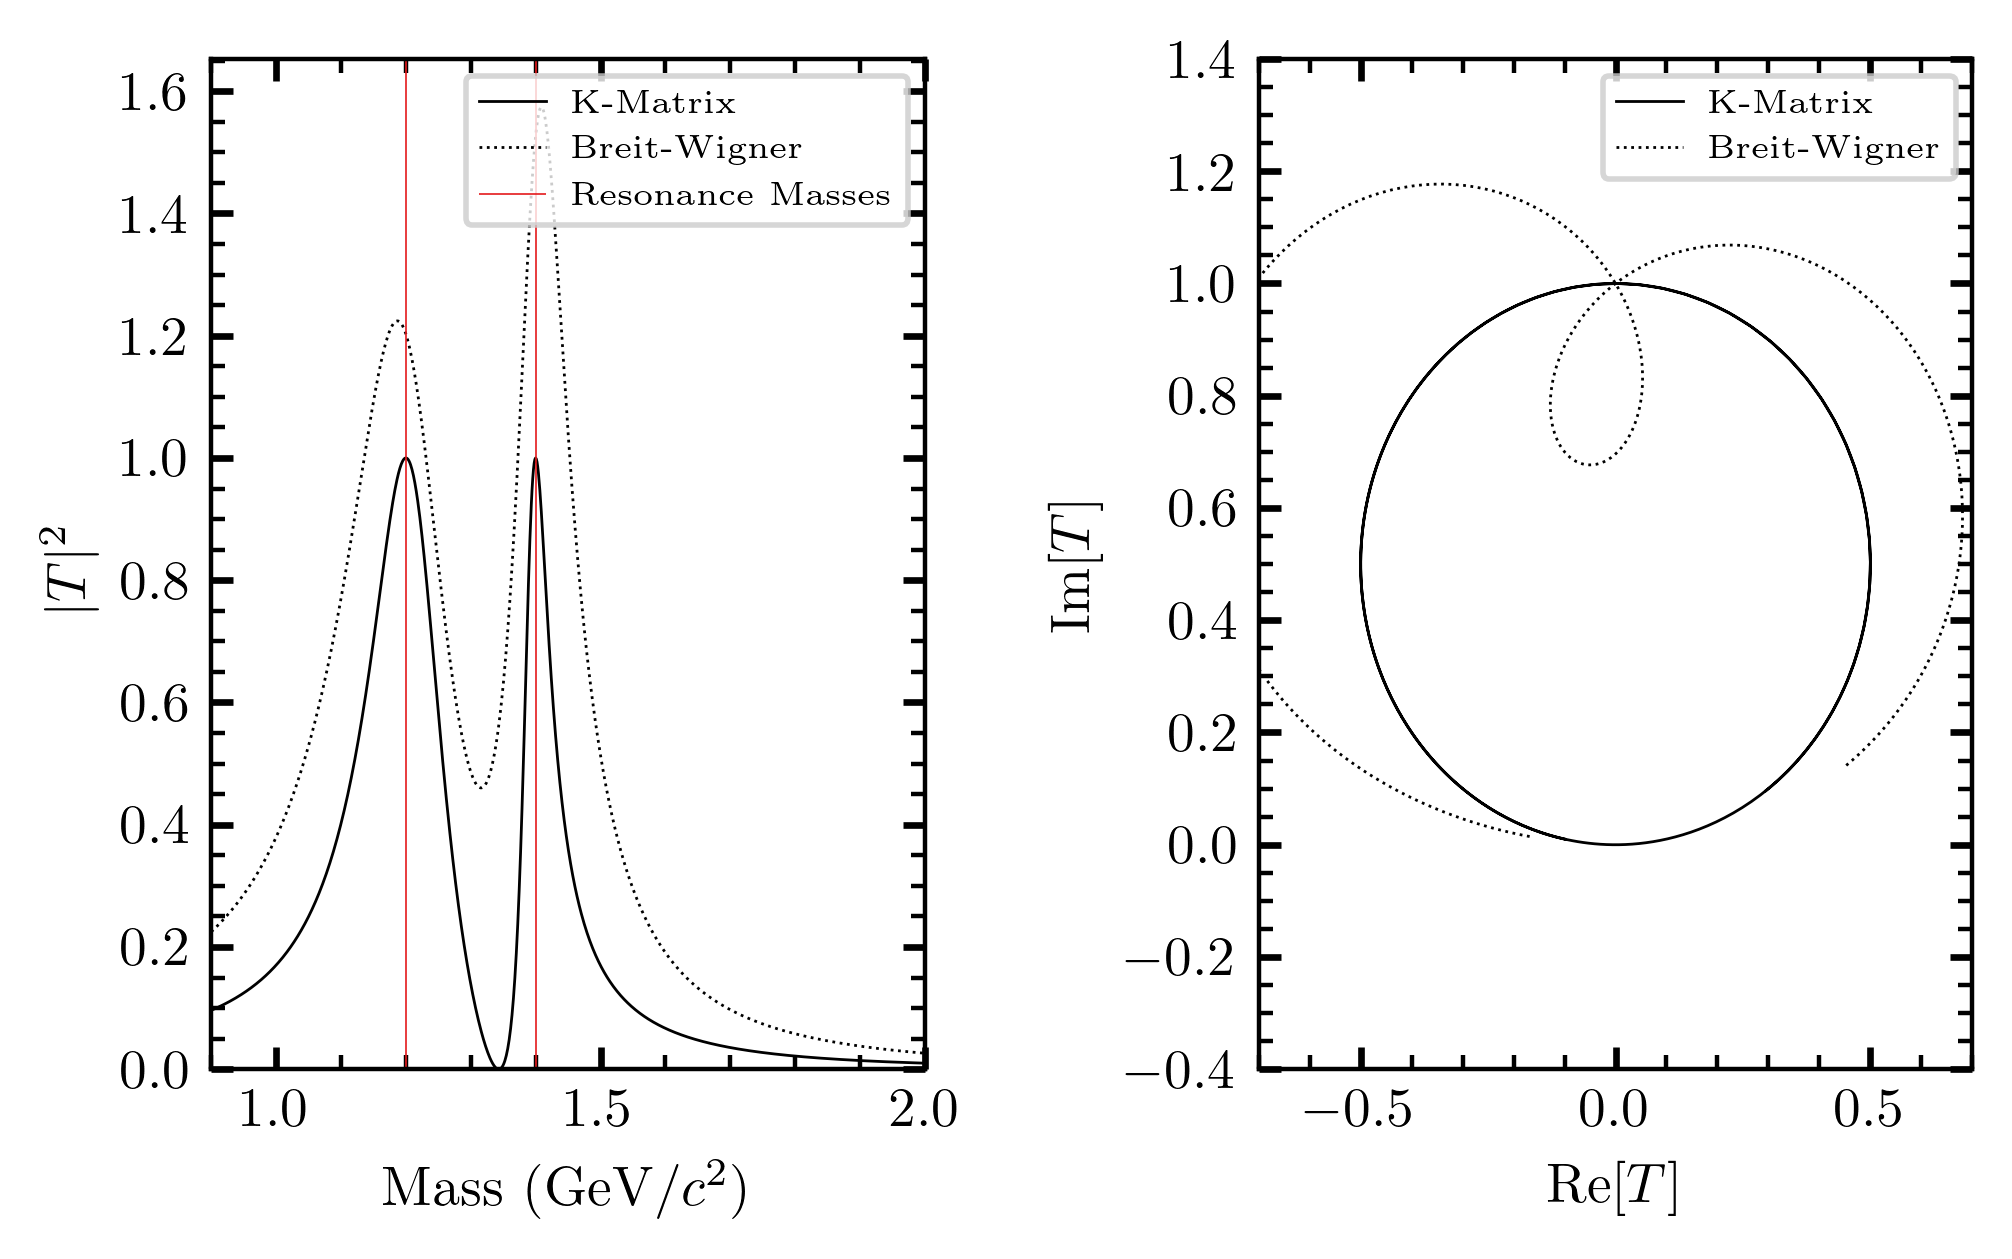
\includegraphics[width=0.8\textwidth]{ext/analysis/plots/argand_diagram.png}
  \end{center}
  \caption{An Argand diagram depicting two fictitious resonances with masses of $\SI{1.2}{\giga\eV}/c^2$ and $\SI{1.4}{\giga\eV}/c^2$ and widths of $\SI{200}{\mega\eV}/c^2$ and $\SI{100}{\mega\eV}/c^2$ respectively using both the $K$-matrix formalism and interfering Breit-Wigners. The $T$-matrix formed from Breit-Wigners exceeds the unitary circle, implying that this construction breaks unitarity, while the $K$-matrix does not.}\label{fig:argand-diagram}
\end{figure}

\subsection{Resonances as Poles of the $K$-matrix}

Resonances can be parametrized either as constant elements in the $K$-matrix, which are usually interpreted as ``molecular'' resonances resulting from the exchange of force-carrying bosons, or from poles, which are thought of as the resonances describing decaying hadrons~\cite{Au1987}. While we are more interested in the second case, we will include a linear combination of poles and constant terms in the parameterization, as follows:

\begin{equation}
  K_{ij}(m) = \sum_{\alpha} \frac{g_{\alpha i}(m) g_{\alpha j}(m)}{m_\alpha^2 - m^2} + c_{ij}
  \label{eq:k-matrix-parameterization}
\end{equation}

Here, $\alpha$ indexes the resonances, with $m_\alpha$ corresponding to the pole mass\footnote{This is not necessarily the same value as the centroid of a Breit-Wigner fit to the same data.} of the $\alpha$th resonance and $g_{\alpha i}$ corresponding to a term coupling the $\alpha$th resonance to the $i$th decay channel. $c_{ij}$ denotes any constant (molecular) terms mentioned previously.

For a single resonance in a single channel, we can write the $T$-matrix as

\begin{align}
  T &= K(I-\imath K)^{-1} \\
    &= \frac{\frac{g^2(m)}{m_\alpha^2 - m^2}}{1 - \imath \left(\frac{g^2(m)}{m_\alpha^2 - m^2}\right)} \\
    &= \frac{g^2(m)}{m_\alpha^2 - m^2 - \imath g^2(m)},
\end{align}
which we see is identical to the Breit-Wigner form given in \Cref{eq:breit-wigner} with $g^2(m) = m_\alpha\Gamma_\alpha(m)$\footnote{Here, $\Gamma$ depends on $m$, which is true for a relativistic form of the Breit-Wigner amplitude.}.

Furthermore, we can now demonstrate the fundamental reason why we need to use the $K$-matrix in lieu of Breit-Wigners when describing multiple overlapping resonances. \Cref{fig:argand-diagram} shows that, even in a single channel, two interfering Breit-Wigners do not preserve unitarity, while the corresponding $K$-matrix does.

In the case where a resonance can decay into multiple channels, we say that $\Gamma_\alpha(m) = \sum_i \Gamma_{\alpha i}(m)$ is the total width and $\Gamma_{\alpha i}(m)$ are called the partial widths. In the relativistic form of the Breit-Wigner (and the Lorentz-invariant form of the resulting $S$-matrix), widths (and therefore partial widths) are given by

\begin{equation}
  \Gamma_{\alpha i} = \gamma^2_{\alpha i} \Gamma_{\alpha} B^\ell_{\alpha i}(m) \sqrt{\rho_i(m)},
  \label{eq:partial-width}
\end{equation}
where $\gamma^2_{\alpha i}$ is the fraction of the total width\footnote{However, $\gamma_{\alpha i}$ may itself be negative so long as it is purely real.}, $\Gamma_\alpha$, which is coupled to the channel $i$, and $\rho_i(m)$ is the phase space factor

\begin{equation}
  \rho_i(m) = \sqrt{\chi^+_i(m)\chi^-_i(m)},\quad\text{where}\quad\chi^{\pm}_i = 1 - \left(\frac{m_1 \pm m_2}{m}\right)^2.
  \label{eq:rho}
\end{equation}

Here, the $i$th channel describes the decay $\alpha \to 1 + 2$ and $B^\ell_{\alpha i}(m)$ is the centrifugal barrier factor describing the suppression to the partial width when a resonance has angular momentum $\ell$. We typically parameterize this via form factors derived by Blatt and Weisskopf~\cite{Blatt1979}:

\begin{align}
  B^\ell_{\alpha i}(m) &= \frac{F_\ell(z_i(m))}{F_\ell(z_i(m_\alpha))} \\
  z_i(m) &\equiv \left(\frac{q_i(m)}{q_R}\right)^2 \\
  F_0(z) &= 1 \\
  F_1(z) &= \sqrt{\frac{2z}{z+1}} \\
  F_2(z) &= \sqrt{\frac{13z^2}{(z-3)^2 + 9z}} \\
  F_\ell(z) &= \sqrt{\frac{\abs{h_\ell^{(1)}(1)}^2}{z\abs{h_\ell^{(1)}(\sqrt{z})}^2}},
\end{align}
where $q_i(m) = m\rho_i(m)/2$ is the breakup momentum for the $i$th channel\footnote{i.e. the magnitude of the momentum either decay product will have in the rest frame of the decay}, $q_R$ is the impact parameter/interaction radius (we use $\SI{0.1973}{\giga\eV}$ in our calculations), and $h_\ell^{(1)}$ is a spherical Hankel function of the first kind (see Equation 2.4 of~\cite{vonHippel1972})

For clarity, we typically reparameterize these partial widths such that

\begin{equation}
  g_{\alpha i}(m) = g_{\alpha i}B^\ell_{\alpha i}(m)\sqrt{\rho_i(m)},
  \label{eq:coupling-expansion}
\end{equation}
so we can define the Lorentz-invariant $K$-matrix, $\hat{K}$, as

\begin{align}
  K_{ij}(m) &= \sqrt{\rho_i(m)}\left(\sum_{\alpha}B^\ell_{\alpha i}(m)\left[\frac{g_{\alpha i}g_{\alpha j}}{m_\alpha^2 - m^2} + \sum_n \bar{c}_{nij} m^{2n}\right]B^\ell_{\alpha j}\right)\sqrt{\rho_j(m)} \notag\\
  K_{ij}(m) &= \sqrt{\rho_i(m)} \hat{K}_{ij}(m) \sqrt{\rho_j(m)},
  \label{eq:invariant-k-matrix}
\end{align}
where we have absorbed some multiplicative factors into $c_{ij}$ to form the series expansion over powers of $m^2$ (since $\rho(m)$ and $B^\ell_{\alpha i}(m)$ only contain even powers of $m$) with coefficients $\bar{c}_{ij}$. Here, $\hat{K}$ replaces $K$ in \Cref{eq:t-matrix-from-k-matrix} as an intermediate step to defining a Lorentz-invariant formulation.

According to Chung~\cite{Chung1971}, the Lorentz-invariant form of the $T$-matrix, $\hat{T}$ can be written as

\begin{equation}
  T = \sqrt{\rho}\hat{T}\sqrt{\rho},
\end{equation}
where we define the notation

\begin{align}
  \rho_{ij}(m) &\equiv \rho_i(m)\delta_{ij}\\
  (\sqrt{\rho})_{ij} = \sqrt{\rho_{ij}(m)} &\equiv \sqrt{\rho_i(m)}\delta_{ij}.
\end{align}

In terms of \Cref{eq:t-matrix-from-k-matrix,eq:invariant-k-matrix,eq:k-t-inverse-relation}, we can write

\begin{equation}
  \hat{K}^{-1} = \hat{T}^{-1} + \imath \rho.
\end{equation}

Following the previous derivation with these invariant forms, we find that

\begin{equation}
  \hat{T} = (I - \imath\hat{K}\rho)^{-1}\hat{K}.
  \label{eq:t-matrix-from-k-matrix-invariant}
\end{equation}


\subsubsection{Production Amplitudes from a $K$-Matrix}

The $T$-matrix given in \Cref{eq:t-matrix-from-k-matrix-invariant} describes $s$-channel resonances (as in $a + b \to X \to c + d$). We can transform this into a production amplitude following Aitchison~\cite{Aitchison1972}:

\begin{equation}
  \hat{F} = (I - \imath\hat{K}\rho)^{-1}\hat{P},
  \label{eq:k-matrix-production-amplitude}
\end{equation}
where
\begin{equation}
  \hat{P}_i(\vec{\beta}; m) = \sum_\alpha \left(\frac{\beta_\alpha g_{\alpha i}}{m_\alpha^2 - m^2} + \sum_n c_{ni} m^{2n} \right)B_{\alpha i}^{\ell}(m).
  \label{eq:p-vector}
\end{equation}

Here, $\beta_\alpha$ describes the complex coupling from the initial state to the resonance $\alpha$. This can be thought of like a coupling coefficient in front of a single Breit-Wigner. The polynomial of coefficients are included for completeness, as any constant terms in $P$ preserve unitarity in the same way as constant terms in $K$, and the division of the factor of $\rho_i(m) \sim \rho_i(m^2)$ from \Cref{eq:coupling-expansion} and $B^\ell_{\alpha i}(m) \sim B^\ell_{\alpha i}(m^2)$ creates the given form.

\subsubsection{The Chew-Mandelstam Matrix}

For reasons which will become clear, we will define the diagonal matrix $C$, called the Chew-Mandelstam matrix, with the property

\begin{equation}
  \Im[C(m)] = -\rho(m)\quad\text{or}\quad C(m) = A(m) - \imath\rho(m)
\end{equation}
for some real function $A(m)$. It can be shown that we can replace $-\imath\rho$ in \Cref{eq:t-matrix-from-k-matrix-invariant} with such a matrix $C$ and still retain a valid $K$-matrix representation~\cite{Wilson2015},

\begin{equation}
  \hat{T} = (I + \hat{K}C)^{-1}\hat{K}
\end{equation}
and

\begin{equation}
  \hat{F} = (I + \hat{K}C)^{-1}\hat{P}.
  \label{eq:k-matrix-production-amplitude-chew}
\end{equation}

The exact form of $A(m)$ is arbitrary, but we will be using

\begin{equation}
  C_{ii}(m) = C((m_1 + m_2)^2) + \frac{\rho_i(m)}{\pi}\ln\left[\frac{\chi^+_i(m) + \rho_i(m)}{\chi^+_i(m) - \rho_i(m)}\right] - \frac{\chi^+_i(m)}{\pi}\frac{m_2 - m_1}{m_1 + m_2}\ln\frac{m_2}{m_1},
  \label{eq:chew-mandelstam}
\end{equation}
where $m_1$ and $m_2$ are the masses of the final state of the $i$th decay channel, and we can choose $C((m_1 + m_2)^2) = 0$ for normalization. See~\cite{Oller1999},~\cite{Basdevant1977},~\cite{Oller2001}, and~\cite{Reid1984} for derivations and additional details of this expression. The motivation for this choice is that it behaves better below threshold than $\rho(m)$, as can be seen in \Cref{fig:chew-mandelstam}.

\begin{figure}
  \begin{center}
    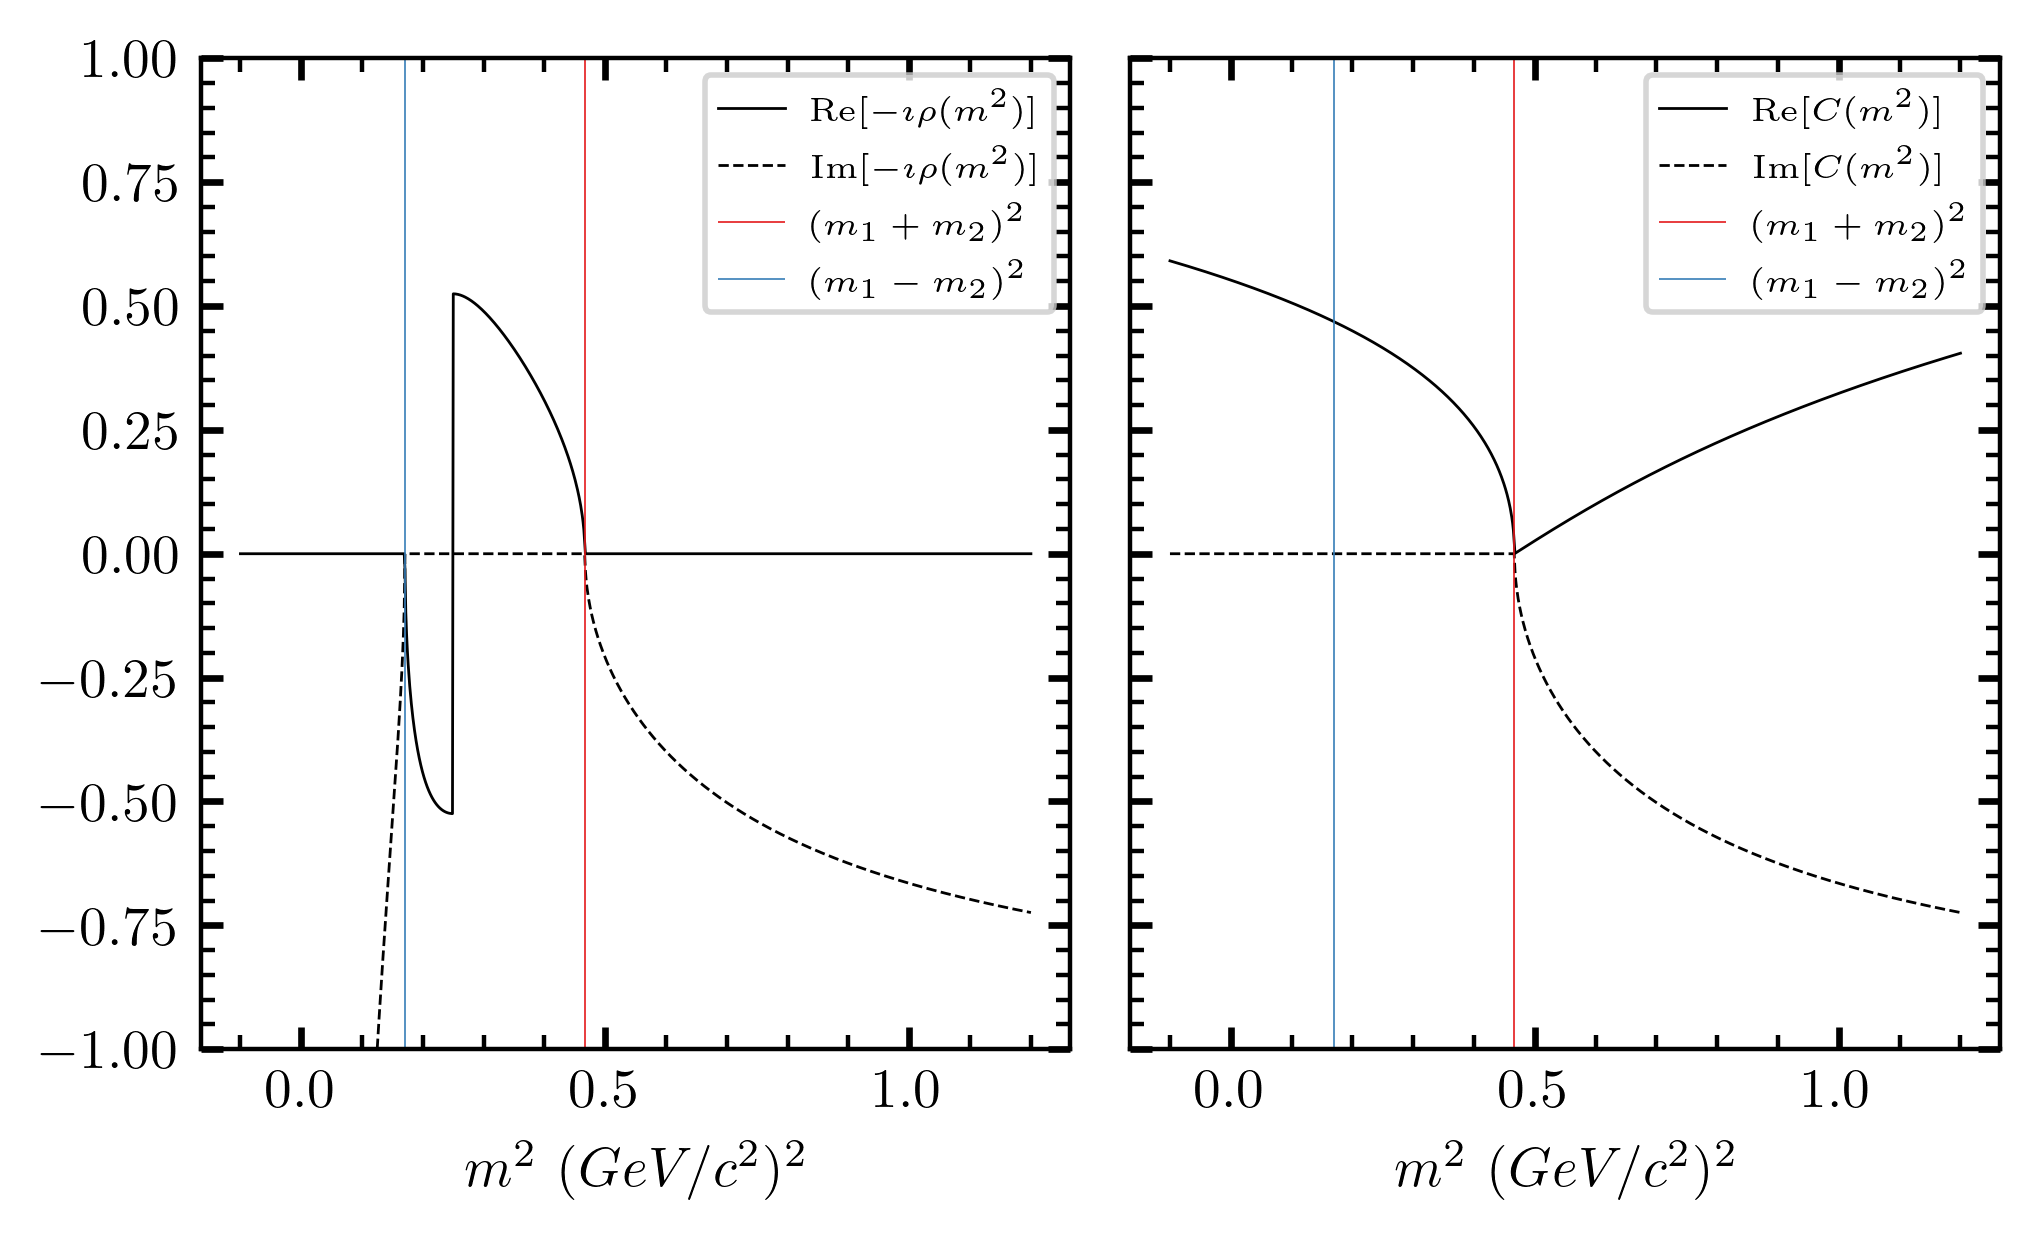
\includegraphics[width=0.8\textwidth]{ext/analysis/plots/chew_mandelstam.png}
  \end{center}
  \caption{A comparison of the normal phase-space function, $\rho(m)$ (left) and the Chew-Mandelstam matrix, $C(m)$ (right) on the $\pi^0\eta$ channel. Both functions have the same imaginary part above the threshold $m = m_1 + m_2$, but the phase-space function has a branch cut at $m^2 = \frac{(m_1^2 - m_2^2)^2}{m_1^2 + m_2^2}$ (the jump in the left plot between the red and blue lines) as well as a discontinuity at $m^2 = (m_1 - m_2)^2$ in both real and imaginary parts.}\label{fig:chew-mandelstam}
\end{figure}


The impetus of this complication is that this particular formulation of the Chew-Mandelstam matrix is used in~\cite{Albrecht2020} and~\cite{Kopf2021}. We do not have enough data to constrain the pole positions of every resonance in this channel (as we only have access to one of several channels used in those papers), so we will use the $K$-matrix coefficients ($g_{i\alpha}$ and $m_\alpha$) from their coupled-channel analysis of data from the Crystal Barrel and COMPASS experiments as fixed values in our analysis, fitting only the couplings ($\vec{\beta}$) to photoproduction. Additionally, using the results from these papers requires a Adler zero term in front of the $K$-matrix for the $f_0$ mesons of the form $\frac{(s - s_0)}{s_\text{norm}}$, where they use $s_0 = m^2_{\pi_0}/2$ and $s_\text{norm} = 1$.

We can then combine \Cref{eq:k-matrix-production-amplitude-chew} with \Cref{eq:generalized-polarized-intensity}, choosing $T^{J(\epsilon)}_{M;\eta}(\vec{\beta}; m) = \hat{F}(\vec{\beta}; m)$, to form a mass-dependent model of polarized photoproduction for the $K_S^0K_S^0$ channel which will be further discussed in \Cref{sec:mass-dependent-fits}.
